\section{A Basic KAC Using Asymmetric Bilinear Pairings}
\label{sec:proposal}


In this section, we present the design of the basic key-aggregate cryptosystem. Our construction is based on asymmetric bilinear pairings that are practical and efficiently implementable and do not require non-singular elliptic curves. In this respect, our const For the basic case, we assume a single data owner who stores her data in $n$ different classes, with no hierarchical organization within each class. In later discussions, we show how the system can be scaled to multiple users, and also to allow hierarchical constructions within each class. Our scheme ensures that the ciphertext and aggregate key are of constant size, while the public parameter size is linear in the number of data classes $n$. We prove the scheme to non-adaptively CPA secure under the asymmetric $l$-BDHE exponent assumption.

\subsection{Construction}
\label{subsec:construction1}

We present the basic construction of our proposed KAC. As mentioned in Section \ref{sec:prelims}, we assume the existence of equi-prime order (for a $\lambda$-bit prime $q$) elliptic curve subgroups $\mathbb{G}_1$ and $\mathbb{G}_2$, along with their generators $P$ and $Q$. We also assume the existence of a multiplicative cyclic group $\mathbb{G}_{T}$, also of order $q$ with identity element $1$. Finally, we assume there exists an asymmetric bilinear pairing ${e}:\mathbb{G}_1 \times \mathbb{G}_2\longrightarrow\mathbb{G}_T$. The notations used in the forthcoming discussion are already introduced in Section \ref{sec:prelims}.\\

% \begin{enumerate}
 \noindent \textbf{SetUp}$(1^{\lambda},n)$: Randomly pick $\alpha \in \mathbb{Z}_q$. Output the system parameter as $param = (P,Q,Y_{P,\alpha,n},Y_{Q,\alpha,n})$. Discard $\alpha$. \\
 
 \noindent \textbf{KeyGen}(): Randomly pick $\gamma\in \mathbb{Z}_q$. Set the master secret key $msk$ to $\gamma$. Let $PK_1=\gamma P$ and $PK_2=\gamma Q$. Set the public key $PK=(PK_1,PK_2)$. Output $(msk,PK)$.\\
 
 \noindent \textbf{Encrypt}$(param,PK,i,\mathcal{M})$: For a message $\mathcal{M} \in \mathbb{G}_T$ belonging to class $i \in \{1,2,\cdots,n\}$, randomly choose $t\in\mathbb{Z}_q$. Output the ciphertext $\mathcal{C}$ as 
 \begin{equation}
 \mathcal{C}=(tQ,t(PK_2+Q_i),\mathcal{M}.{e}(P_n,tQ_1)) \nonumber
 \end{equation}
 
 \noindent \textbf{Extract}$(param,msk,\mathcal{S})$: For the subset of class indices $\mathcal{S}$, the aggregate key is computed as 
 \begin{equation}
 K_{\mathcal{S}} = {msk}\sum_{j\in\mathcal{S}}P_{n+1-j} \nonumber
 \end{equation} 
 \noindent Note that this is indirectly equivalent to setting $K_{\mathcal{S}}$ to $\sum_{j\in\mathcal{S}}\alpha^{n+1-j}PK_1$.\\
 
 \noindent \textbf{Decrypt}$(param,\mathcal{C},i,K_{\mathcal{S}})$: Let $\mathcal{C}=(c_0,c_1,c_2)$. If $i\notin\mathcal{S}$, output $\bot$. Otherwise, set 
 \begin{eqnarray} 
 a_{\mathcal{S}}&=&\sum_{j\in\mathcal{S},j\neq i}P_{n+1-j+i} \nonumber \\
 b_{\mathcal{S}}&=&\sum_{j\in\mathcal{S}}P_{n+1-j} \nonumber 
 \end{eqnarray} 
 \noindent and return the decrypted message $\hat{\mathcal{M}}$ as: 
 \begin{equation}
  \hat{\mathcal{M}}=c_2.\frac{{e}(K_{\mathcal{S}}+a_{\mathcal{S}},c_0)}{{e}(b_{\mathcal{S}},c_1)} \nonumber
 \end{equation}

% \end{enumerate}

\noindent The proof of correctness of the basic KAC scheme is presented next.

\begin{scriptsize}
\begin{equation*}
\label{eq:correctness}
\begin{split}
 \hat{\mathcal{M}} &= c_2.\frac{{e}(K_{\mathcal{S}}+\sum_{j\in\mathcal{S},j\neq i}P_{n+1-j+i},c_0)}{{e}(\sum_{j\in\mathcal{S}}P_{n+1-j},c_1)}\\
  &= c_2.\frac{{e}(\sum_{j\in \mathcal{S}}{\gamma}P_{n+1-j} + \sum_{j\in\mathcal{S},j\neq i}P_{n+1-j+i},tQ)}{{e}(\sum_{j\in\mathcal{S}}P_{n+1-j},t(PK_2+Q_i))}\\
  &= c_2.\frac{{e}(\sum_{j\in \mathcal{S}}{\gamma}P_{n+1-j},tQ){e}(\sum_{j\in\mathcal{S}}(P_{n+1-j+i})-P_{n+1},tP)}{{e}(\sum_{j\in\mathcal{S}}P_{n+1-j},tPK_2){e}(\sum_{j\in\mathcal{S}}P_{n+1-j},tQ_i))}\\
  &= c_2.\frac{{e}(\sum_{j\in\mathcal{S}}P_{n+1-j+i},tQ)}{{e}(P_{n+1},tQ){e}(\sum_{j\in\mathcal{S}}P_{n+1-j},tQ_i))}\\
  &= c_2.\frac{{e}(\sum_{j\in\mathcal{S}}P_{n+1-j+i},tQ)}{{e}(P_{n+1},tQ){e}(\sum_{j\in\mathcal{S}}P_{n+1-j+i},tQ))}\\
  &= \mathcal{M}.\frac{{e}(P_n,tQ_1)}{{e}(P_{n+1},tQ)}\\
  &= \mathcal{M}
\end{split}  
\end{equation*}
\end{scriptsize}


\subsection{Performance and Efficiency}
\label{subsec:perf_basic}
The decryption time for any subset of ciphertext classes $\mathcal{S}$ is essentially dominated by the computation of $W_{\mathcal{S}}=\sum_{j\in\mathcal{S}}P_{n+1-j+i}$. However, if a user has already computed $\sum_{j\in\mathcal{S}'}P_{n+1-j+i}$ for a subset $S'$ similar to $S$, then she can easily compute the desired value by at most $|\mathcal{S}-\mathcal{S}'|$ operations. For similar subsets $S$ and $S'$, this value is expected to be fairly small. As suggested in \cite{boneh2005collusion}, for subsets of very large size($n-r, r\ll n$), an advantageous approach could be to pre-compute $\sum_{j=1}^{j=n}P_{n+1-j+i}$ corresponding to $i=1$ to $n$, which would allow the user to decrypt using only $r$ group operations, and would require only $r$ elements of $param$. Similar optimizations would also hold for the encryption operation where pre-computation of  $\sum_{j=1}^{j=n}P_{n+1-j}$ is useful for large subsets.



\subsection{Semantic Security of the Basic KAC}
\label{subsec:proof_basic}

We now formally prove the CPA security of the basic KAC. We begin by stating the following theorem.

\begin{Theorem}
\label{th:basicCPA}
Let $\mathbb{G}_1$ and $\mathbb{G}_2$ be bilinear elliptic curve subgroups of prime order $q$. For any pair of positive integers $n',n (n'>n)$, the basic KAC is $(\tau,\epsilon,n')$ CPA secure if the asymmetric decision $(\tau,\epsilon,n)$-BDHE assumption holds in $(\mathbb{G}_1,\mathbb{G}_2)$.
\end{Theorem}

\noindent{\textit{Proof:}} Let $\mathcal{A}$ be a $\tau$-time adversary such that $|Adv_{\mathcal{A},n'}-\frac{1}{2}| > \epsilon$ for a KAC system parameterized with a given $n$. We build an algorithm $\mathcal{B}$ that has advantage at least $\epsilon$ in solving the asymmetric $n$-BDHE problem in $(\mathbb{G}_1,\mathbb{G}_2)$. Algorithm $\mathcal{B}$ takes as input a random asymmetric $n$-BDHE challenge $(I=(H,P,Q,Y_{P,\alpha,n},Y_{Q,\alpha,n}),Z)$ (where $Z$ is either ${e}(P_{n+1},H)$ or a random value in $\mathbb{G}_T$), and proceeds as follows.\\

% \begin{enumerate}
\noindent \textbf{Init:} $\mathcal{B}$ runs $\mathcal{A}$ and receives the set $\mathcal{S}$ of ciphertext classes that $\mathcal{A}$ wishes to be challenged on. $\mathcal{B}$ then randomly chooses a ciphertext class $i\in\mathcal{S}$.\\
 
\noindent \textbf{SetUp}: $\mathcal{B}$ should generate the public $param$ and the public key $PK$  and provide them to $\mathcal{A}$. They are generated as follows.
%  \vspace{-0.6mm}
\begin{itemize}
  \item $param$ is set as $((P,Q,Y_{P,\alpha,n},Y_{Q,\alpha,n}))$.
%   \item $msk$ is set as some $\gamma$ randomly chosen from $\mathbb{Z}_q$.
  \item Set $PK=(PK_1,PK_2)$, where $PK_1$ and $PK_2$ are computed as $\gamma P - P_i$ and $\gamma Q-Q_i$ respectively, for some $\gamma$ randomly chosen from $\mathbb{Z}_q$. Note that this is equivalent to setting $msk$ as $\gamma-\alpha^i$.
  
\end{itemize}
 
\noindent $\mathcal{B}$ computes the collusion aggregate key $K_{\overline{\mathcal{S}}}$ as   
\begin{equation}
 K_{\overline{\mathcal{S}}} = \sum_{j\notin\mathcal{S}}({u}P_{n+1-j}-(P_{n+1-j+i})) \nonumber
\end{equation}

\noindent and provides it to $\mathcal{A}$. Note that this is indirectly equivalent to setting 
\begin{equation}
K_{\overline{\mathcal{S}}}=\sum_{j\notin\mathcal{S}}\alpha^{n+1-j}PK_1\nonumber
\end{equation}
\noindent as desired. Moreover, $\mathcal{B}$ is aware that $i\notin \overline{\mathcal{S}}$ (implying $i\neq j$), and hence has all the resources to compute $K_{\overline{\mathcal{S}}}$.

Since $P$, $Q$, $\alpha$ and $\gamma$ values are chosen uniformly at random, \emph{the public parameters and the public key have an identical distribution to that in the actual construction}.\\
 
\noindent \textbf{Challenge}: $\mathcal{A}$ picks at random two messages $\mathcal{M}_0$ and $\mathcal{M}_1$ from the set of possible plaintext messages in class $i$, and gives them to $\mathcal{B}$. To generate the challenge, $\mathcal{B}$ randomly picks $b\in\{0,1\}$, and sets the challenge as $(\mathcal{C},\mathcal{M}_0,\mathcal{M}_1)$, where $\mathcal{C}=(H,\gamma H,\mathcal{M}_b.Z)$. We claim that when $Z={e}(P_{n+1},H)$ (i.e. the input to $\mathcal{B}$ is a valid asymmetric $n$-BDHE tuple), then $(\mathcal{C},\mathcal{M}_0,\mathcal{M}_1)$ is a valid challenge to $\mathcal{A}$ as in a real attack. To see this, write $H=tQ$ for some unknown $t\in\mathbb{Z}_q$. Then we have 
\begin{eqnarray}
\gamma H&=& t(\gamma Q)=t(PK_2+Q_i)\nonumber \\
\mathcal{M}_b.Z&=&\mathcal{M}_b{e}(P_{n+1},tQ)\nonumber
\end{eqnarray}

\noindent Thus, by definition, $\mathcal{C}$ is a valid encryption of the message $\mathcal{M}_b$ in class $i$ and hence, $(\mathcal{C},\mathcal{M}_0,\mathcal{M}_1)$ is a valid challenge to $\mathcal{A}$. \\
 
\noindent \textbf{Guess}: The adversary $\mathcal{A}$ outputs a guess $b'$ of $b$. If $b' = b$, $\mathcal{B}$ outputs $0$ (indicating that $Z = {e}(P_{n+1},H)$). Otherwise, it outputs $1$ (indicating that $Z$ is a random element in $\mathbb{Z}_T$).\\
% \end{enumerate}

\noindent We now analyze the probability that $\mathcal{B}$ gives a correct output. If $(I,Z)$ is sampled from ${\mathcal{R}'}_{\text{BDHE}}$, we have $Pr[\mathcal{B}(I,Z)=0]$ = $\frac{1}{2}$, while if $(I,Z)$ is sampled from ${\mathcal{L}'}_{\text{BDHE}}$, $|Pr[\mathcal{B}(I,Z)]-\frac{1}{2}|$ = $|Adv_{\mathcal{A},n'}-\frac{1}{2}|$ $\geq$ $\epsilon$. This implies that $\mathcal{B}$ has advantage at least $\epsilon$ in solving the asymmetric $n$-BDHE problem in $(\mathbb{G}_1,\mathbb{G}_2)$. This concludes the proof of Theorem \ref{th:basicCPA}. Note that the proof does not require the use of random oracles. \hfill\qed




\section{Extended KAC with Aggregate Key Broadcast}
\label{sec:extendedconstruction}

In this section, we present a construction for the extended KAC with public-key based aggregate key broadcast introduced in \ref{subsec:extendedKAC}. Our construction efficiently combines the basic KAC instance presented in \ref{subsec:construction1} with the public key based broadcast encryption system presented in \cite{boneh2005collusion} to handle $n$ data classes and $m$ users .\\

% \begin{enumerate}
 \noindent \textbf{SetUp}$(1^{\lambda},n,m)$: Randomly pick $\alpha_1,\alpha_2 \in \mathbb{Z}_q$. Output the system parameter as 
 \begin{equation}
  param = (P,Q,Y_{P,\alpha_1,n},Y_{Q,\alpha_1,n},Y_{P,\alpha_2,m},Y_{Q,\alpha_2,m}) \nonumber
 \end{equation}
 \noindent Discard $\alpha_1$ and $\alpha_2$. Note that in the forthcoming discussion, $P_i={\alpha^i_1} P$ and $\hat{P}_i={\alpha^i_2} P$. Similar definitions follow for $Q_i$ and $\hat{Q}_i$ respectively.\\
 
 \noindent \textbf{OwnerKeyGen}(): Randomly pick $\gamma_1,\gamma_2,\gamma_3\in \mathbb{Z}_q$. Let $msk_1=\gamma_1$ and $msk_2=\gamma_2$. Set the master secret key $msk$ to $(msk_1,msk_2)$. Let $PK_1=\gamma_1 P$, $PK_2=\gamma_1 Q$, $PK_3=\gamma_2 P$ and $PK_4=\gamma_2 Q$. Set the public key $PK=(PK_1,PK_2,Pk_3,PK_4)$. Finally set the broadcast secret key $bsk=\gamma_3$. Output $(msk,PK,bsk)$.\\
 
 \noindent \textbf{Encrypt}$(param,PK,bsk,i,\mathcal{M})$: For a message $\mathcal{M} \in \mathbb{G}_T$ belonging to class $i \in \{1,2,\cdots,n\}$, randomly choose $t\in\mathbb{Z}_q$. Output the ciphertext $\mathcal{C}$ as:
 \begin{equation}
 \mathcal{C}=(tQ,(t-bsk)PK_2,t(PK_2+Q_i),\mathcal{M}.{e}(P_n,tQ_1)) \nonumber
 \end{equation}
 
 \noindent \textbf{UserKeyGen}$(param,msk,\hat{i})$: Output the private key for user with id $\hat{i}$ as: 
 \begin{equation}
  d_{\hat{i}} = msk_2{\hat{P}}_{\hat{i}} \nonumber\\
 \end{equation}
 \noindent Note that this is indirectly equivalent to setting $d_{\hat{i}}$ to $\alpha^{\hat{i}}PK_3$.\\
 
 \noindent \textbf{Extract}$(param,msk,\mathcal{S})$: For the subset of class indices $\mathcal{S}$, the aggregate key is computed as: 
 \begin{equation}
 K_{\mathcal{S}} = {msk}\sum_{j\in\mathcal{S}}P_{n+1-j} \nonumber
 \end{equation} 
 \noindent Note that this is indirectly equivalent to setting $K_{\mathcal{S}}$ to $\sum_{j\in\mathcal{S}}\alpha^{n+1-j}PK_1$.\\
 
 \noindent \textbf{Broadcast}$(param,K_{\mathcal{S}},\hat{\mathcal{S}},PK,bsk)$:  Broadcasts the aggregate key $K_{\mathcal{S}}$ to all users in $\hat{\mathcal{S}}$ as follows. Randomly choose $\hat{t}\in\mathbb{G}_q$ and set
 \begin{equation}
  \hat{b}_{\hat{\mathcal{S}}}=\sum_{\hat{j}\in\hat{\mathcal{S}}}\hat{Q}_{m+1-\hat{j}} \nonumber 
 \end{equation}
 \noindent Output
 \begin{equation}
  K_{\left(\mathcal{S},\hat{\mathcal{S}}\right)} = (\hat{t}Q,PK_4+\hat{b}_{\hat{\mathcal{S}}},\mathcal{K})\nonumber
 \end{equation}
 \noindent where 
 \begin{equation}
  \mathcal{K}=\left(e(\hat{P}_m,\hat{Q}_1).e(K_{\mathcal{S}},Q)^{bsk}\right)\nonumber\\
 \end{equation}
 \noindent Note that the actual group element corresponding to $K_{\mathcal{S}}$ is difficult to recover from $\mathcal{K}$. However, as we demonstrate next, this knowledge is not explicitly necessary for decryption.\\
 
 \noindent\textbf{Decrypt}$(param,\mathcal{C},K_{\left(\mathcal{S},\hat{\mathcal{S}}\right)},i,\hat{i},d_{\hat{i}},\mathcal{S},\hat{\mathcal{S}})$: If $i\notin\mathcal{S}$ or $\hat{i}\notin\hat{\mathcal{S}}$, output $\bot$. Otherwise, set
 \begin{eqnarray} 
 \hat{a}_{\hat{\mathcal{S}}}&=&\sum_{\hat{j}\in\hat{\mathcal{S}},\hat{j}\neq \hat{i}}\hat{P}_{m+1-\hat{j}+\hat{i}}\nonumber\\
 a_{\mathcal{S}}&=&\sum_{j\in\mathcal{S},j\neq i}P_{n+1-j+i} \nonumber \\
 b_{\mathcal{S}}&=&\sum_{j\in\mathcal{S}}P_{n+1-j} \nonumber 
 \end{eqnarray} 
 \noindent Let $\mathcal{C}=(c_0,c_1,c_2,c_3)$ and $K_{\left(\mathcal{S},\hat{\mathcal{S}}\right)}=(\hat{k}_0,\hat{k}_1,\hat{k}_2)$. Output the decrypted message as  
\begin{eqnarray} 
\hat{\mathcal{M}}&=&c_3.\hat{k}_2.\left(\frac{e(b_{\mathcal{S}},c_1){e}(a_{\mathcal{S}},c_0)}{{e}(b_{\mathcal{S}},c_2)}\right).\left(\frac{e(d_{\hat{i}}+a_{\hat{\mathcal{S}}},\hat{k}_0)}{e(\hat{P}_{\hat{i}},\hat{k}_1)}\right) \nonumber
\end{eqnarray}

\noindent The proof of correctness of the extended KAC scheme is similar to that for the basic construction and is avoided. We now prove static security of the extended scheme in the CPA model.

\subsection{Semantic Security of the Extended KAC}
\label{subsec:proof_extended}

We state the following theorem.

\begin{Theorem}
\label{th:extendedCPA}
Let $\mathbb{G}_1$ and $\mathbb{G}_2$ be bilinear elliptic curve subgroups of prime order $q$. For any pair of positive integers $n',n (n'>n)$ and another pair of positive integers $m',m (m'>m)$, the extended KAC is $(\tau,\epsilon,n',m')$ CPA secure if the asymmetric decision $(\tau,\epsilon,n,m)$-BDHE assumption holds in $(\mathbb{G}_1,\mathbb{G}_2)$.
\end{Theorem}

\noindent{\textit{Proof:}} Let $\mathcal{A}$ be a $\tau$-time adversary such that $|Adv_{\mathcal{A},n',m'}-\frac{1}{2}| > \epsilon$ for a KAC system parameterized with a given pair $(n,m)$. We build an algorithm $\mathcal{B}$ that has advantage at least $\epsilon$ in solving the asymmetric $(n,m)$-BDHE problem in $(\mathbb{G}_1,\mathbb{G}_2)$. Algorithm $\mathcal{B}$ takes as input a random asymmetric $(n,m)$-BDHE challenge $((I_1,I_2),(Z_1,Z_2))$ (where $I_1=(H_1,P,Q,Y_{P,\alpha_1,l_1},Y_{Q,\alpha_1,l_1})$, $I_2=(H_2,P,Q,Y_{P,\alpha_2,l_2},Y_{Q,\alpha_2,l_2})$ and $(Z_1,Z_2)$ is either $\left({e}(P_{n+1},H_1),e(\hat{P}_{m+1},H_2)\right)$ or a random value in $\mathbb{G}_T$), and proceeds as follows.\\

% \begin{enumerate}
\noindent \textbf{Init:} $\mathcal{B}$ runs $\mathcal{A}$ and receives the set $\mathcal{S}$ of data classes and the set $\hat{\mathcal{S}}$ of data users that $\mathcal{A}$ wishes to be challenged on. $\mathcal{B}$ then randomly chooses a ciphertext class $i\in\mathcal{S}$.\\
 
\noindent \textbf{SetUp}: $\mathcal{B}$ sets up the extended KAC system by generating the following:
%  \vspace{-0.6mm}
\begin{itemize}
  \item $param$ is set as 
  \begin{equation}
    param = (P,Q,Y_{P,\alpha_1,n},Y_{Q,\alpha_1,n},Y_{P,\alpha_2,m},Y_{Q,\alpha_2,m})\nonumber   
  \end{equation}
  \noindent and supplied to $\mathcal{A}$.
  \item $\mathcal{B}$ randomly chooses $\gamma_1,\gamma_2\in\mathbb{Z}_q$ and computes the following:
  \begin{eqnarray}
   PK_1 &=& \gamma_1 P - P_i\nonumber\\
   PK_2 &=& \gamma_1 Q - Q_i\nonumber\\
   PK_3 &=& \gamma_2P-\sum_{\hat{j}\in\hat{\mathcal{S}},\hat{j}\neq \hat{i}}\hat{P}_{m+1-\hat{j}}\nonumber\\
   PK_4 &=& \gamma_2Q-\sum_{\hat{j}\in\hat{\mathcal{S}},\hat{j}\neq \hat{i}}\hat{Q}_{m+1-\hat{j}}\nonumber
  \end{eqnarray}
  \noindent $\mathcal{B}$ sets the public key $PK=(PK_1,PK_2,PK_3,PK_4)$ and supplies it to $\mathcal{A}$. Note that this is equivalent to setting the master secret key $msk$ as:
  \begin{equation}
   (msk_1,msk_2)=\left(\gamma_1-\alpha^i_1,\gamma_2-\sum_{\hat{j}\in\hat{\mathcal{S}},\hat{j}\neq \hat{i}}\alpha^{m+1-\hat{j}+\hat{i}}_2\right)\nonumber
  \end{equation}
  \noindent Finally, $\mathcal{B}$ chooses a random $\gamma_3\in\mathbb{Z}_q$ and implicitly sets the value of the secret broadcast key $bsk$ to $t-\gamma_3$, such that $H_1=tQ$. We see later how this implicit definition manifests in the actual game.
  
\end{itemize}
 
\noindent $\mathcal{B}$ also supplies $\mathcal{A}$ with all the secret keys for all users not in $\hat{\mathcal{S}}$. In particular, the key for user $\hat{i}$ is set as:
\begin{equation}
 d_{\hat{i}} = \gamma_2{\hat{P}_{\hat{i}}}-{\sum_{\hat{j}\in\hat{\mathcal{S}},\hat{j}\neq \hat{i}}\hat{P}_{m+1-\hat{j}+\hat{i}}}\nonumber
\end{equation}
\noindent Observe that $d_{\hat{i}}=\alpha^{\hat{i}}PK_3$ as desired. In addition, $\mathcal{A}$ is also supplied with the collusion aggregate key $K_{\left(\overline{\mathcal{S}},\hat{\mathcal{S}}\right)}$. For this, $\mathcal{B}$ first computes

\begin{equation}
 K_{\overline{\mathcal{S}}} = \sum_{j\notin\mathcal{S}}({u}P_{n+1-j}-(P_{n+1-j+i})) \nonumber
\end{equation}
\noindent and sets
\begin{equation}
 \overline{\mathcal{K}} = Z_2.e(K_{\overline{\mathcal{S}}},H_1-\gamma_3Q)\nonumber
\end{equation}
\noindent Note that the implicit definition of $bsk$ is used here. Finally, $\mathcal{B}$ provides $\mathcal{A}$ with the aggregate key:
\begin{equation}
 K_{\left(\overline{\mathcal{S}},\hat{\mathcal{S}}\right)} = (H_2,\gamma_2H_2,\overline{\mathcal{K}})\nonumber
\end{equation}
\noindent It can be easily shown that whenever $Z_2={e}(\hat{P}_{l_2+1},H_2)$, this is a valid collusion aggregate key for the sets $\mathcal{S}$ of data classes and $\hat{\mathcal{S}}$ of user ids.
 
\noindent \textbf{Challenge}: $\mathcal{A}$ picks at random two messages $\mathcal{M}_0$ and $\mathcal{M}_1$ from the set of possible plaintext messages in class $i$, and gives them to $\mathcal{B}$. To generate the challenge, $\mathcal{B}$ randomly picks $b\in\{0,1\}$, and sets the challenge as $(\mathcal{C},\mathcal{M}_0,\mathcal{M}_1)$, where 
\begin{equation}
\mathcal{C}=(H_1,PK_1,\gamma_1 H_1,\mathcal{M}_b.Z_1)\nonumber
\end{equation}
\noindent Once again, it can be easily shown that when $Z_1={e}(P_{n+1},H_1)$, then $(\mathcal{C},\mathcal{M}_0,\mathcal{M}_1)$ is a valid challenge to $\mathcal{A}$ as in a real attack.\\
 
\noindent \textbf{Guess}: The adversary $\mathcal{A}$ outputs a guess $b'$ of $b$. If $b' = b$, $\mathcal{B}$ outputs $0$. Otherwise, it outputs $1$ .\\
% \end{enumerate}

\noindent We conclude that $\mathcal{B}$ has at least the same advantage $\epsilon$ as $\mathcal{A}$ in solving the asymmetric $(n,m)$-BDHE problem in $(\mathbb{G}_1,\mathbb{G}_2)$. This concludes the proof of Theorem \ref{th:basicCPA}. Note that this proof is again in the standard model and does not require the use of random oracles. \hfill\qed

\begin{figure*}
\centering
\captionsetup{font=scriptsize}
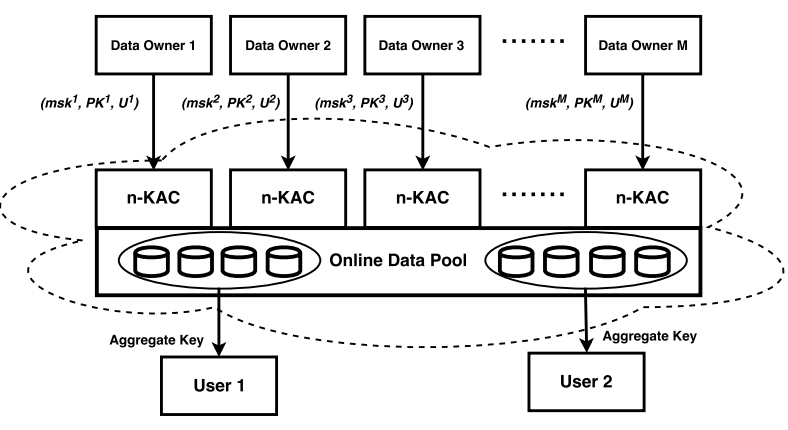
\includegraphics[scale=0.4]{Figs/MultiUser.png}
\caption{Generalized Multi-Data Owner KAC}
\label{fig:two-tier}
\end{figure*}

\subsection{Data Privacy}
\label{subsec:multiownerKAC}

In any online data sharing environment with multiple data owners, data privacy is an essential requirement. In particular, the aggregate key supplied by one data owner should not leak information about another data owner to an unauthorized user. This problem however does not arise in our construction if a new parallel instance of the KAC construction in Section \ref{sec:extendedconstruction}  is run for each data owner. Each instance can handle $n$ data classes and can cater to $m$ data users. In order to distinguish between data classes belonging to different instances, each data class is assigned a double index $(i_1,i_2)$, where $i_1$ is the instance/owner index, and $i_2$ is the class index specific to the instance. Each instance $i_1$ is characterized by its own master secret key $msk^{i_1}$, public key $PK^{i_1}$ and broadcast key $bsk^{i_1}$. The main advantages of this multi-user setup are as follows:

\begin{enumerate}
 \item All the parallel instances can share the same public $param$, which needs to be setup exactly once by the system administrator.
 \item Data privacy is ensured for each individual data owner. In particular, the aggregate key issued by one data owner does not compromise the security of some other owner's data.
 \item The system is scalable since it allows new users to register and share their data without having to alter the underlying basic KAC set-up in any way. This also implies that the basic security assumption of the system is not affected by the increase in the number of data classes.
\end{enumerate}

\noindent Also note that the number of unique ordered tuples $\left(msk^{i_1},PK^{i_1},dsk^{i_1}\right)$ is $q^3$ for the extended construction, meaning that a single setup can support $O(q^3)$ data owners. Finally, if a data owner wishes to store more than $n$ classes of data or cater to more than $n$ data users, she may be allocated more than one instance of the KAC construction in Section \ref{sec:extendedconstruction}. Figure \ref{fig:two-tier} illustrates a practical data sharing scenario with multiple owners sharing their data and distributing access to different users. In summary, the KAC construction is an ideal choice for building a fully public-key based online data sharing scheme.


\subsection{Embedding Plaintext Messages in Bilinear Groups}
\label{subsec:embedding}

The two KAC constructions - basic and extended presented in Sections \ref{sec:proposal} and \ref{sec:extendedconstruction} respectively, assume that all plaintext messages $\mathcal{M}$ may be efficiently embedded as elements in the multiplicative group $G_T$. Unfortunately, embedding any general class of data such as multimedia as elements of a bilinear group is extremely challenging. However, a workaround may be readily proposed. We first note that in any ciphertext output by \textbf{Encrypt}, the message $\mathcal{M}$ is essentially multiplied with a random secret group element $\rho$. Rather than embedding $\mathcal{M}$ as a group element, we propose hashing $\rho$ using a collision resistant hash function $H$, and then outputting $\mathcal{M}\odot H(\rho)$ in the ciphertext (here $\odot$ denotes an appropriate operator). In order to ensure that the constructions are still provably secure in the standard model, we propose that $H$ be chosen from the family of \emph{smooth projective hash functions} \cite{cramer2002universal}, that do not require the use of random oracles to prove security. Smooth projective hash functions are very efficient to construct and can be designed to be collision-resistant \cite{abdalla2009smooth}, making them an ideal choice for our constructions.



Finally, we note that our KAC constructions are agnostic of the manner in which the data owner organizes her data. In particular, our construction is easily adaptable for hierarchical data structures, since a data owner could create an aggregate key corresponding to all the data classes rooted at any internal node, and then broadcast it to the target user group.


  


